\documentclass[11pt]{article}

%------------------------- fonts & encoding -----------------------------------
\usepackage[T1]{fontenc}
\usepackage[utf8]{inputenc}
\usepackage{amsmath,amssymb,amsthm}
\usepackage{mathtools}
\usepackage[sc]{mathpazo}
\linespread{1.06}
\usepackage{microtype}

%------------------------- layout ---------------------------------------------
\usepackage[a4paper,margin=1.05in,marginparwidth=1.0in]{geometry}
\usepackage{booktabs}
\usepackage{enumitem}
\setlist{itemsep=2pt,topsep=3pt}
\usepackage{xcolor}
\usepackage{graphicx}
\usepackage{tikz}
\usepackage{pgfplots}
\pgfplotsset{compat=1.17}
\usepackage[most,breakable]{tcolorbox}

%------------------------- palette --------------------------------------------
\definecolor{crimson}{HTML}{A51C30}
\definecolor{ink}{HTML}{1A1A1A}
\definecolor{steel}{HTML}{2C5F8A}
\definecolor{amber}{HTML}{9A6A00}
\definecolor{teal}{HTML}{1F6F6B}
\definecolor{paperlt}{HTML}{F7F4EF}

%------------------------- section styling ------------------------------------
\usepackage{titlesec}
\titleformat{\section}{\Large\bfseries\color{steel}}{\thesection}{0.7em}{}
\titleformat{\subsection}{\large\bfseries\color{ink}}{\thesubsection}{0.6em}{}
\titlespacing*{\section}{0pt}{1.6em}{0.6em}

%------------------------- hyperref -------------------------------------------
\usepackage[colorlinks=true,linkcolor=steel,citecolor=steel,urlcolor=crimson]{hyperref}

%------------------------- theorem environments -------------------------------
\theoremstyle{definition}
\newtheorem{definition}{Definition}[section]
\newtheorem{example}{Example}[section]
\newtheorem{exercise}{Exercise}[section]
\theoremstyle{plain}
\newtheorem{proposition}{Proposition}[section]
\theoremstyle{remark}
\newtheorem*{remark}{Remark}

%------------------------- callout boxes --------------------------------------
\newtcolorbox{intuition}{
  enhanced, breakable, colback=crimson!5, colframe=crimson, boxrule=0.4pt,
  left=8pt,right=8pt,top=6pt,bottom=6pt, arc=2pt,
  borderline west={2.5pt}{0pt}{crimson},
  fonttitle=\bfseries\color{crimson}, title={Intuition}}

\newtcolorbox{pitfall}{
  enhanced, breakable, colback=amber!7, colframe=amber, boxrule=0.4pt,
  left=8pt,right=8pt,top=6pt,bottom=6pt, arc=2pt,
  borderline west={2.5pt}{0pt}{amber},
  fonttitle=\bfseries\color{amber}, title={What goes wrong}}

\newtcolorbox{keyresult}{
  enhanced, breakable, colback=steel!6, colframe=steel, boxrule=0.5pt,
  left=8pt,right=8pt,top=6pt,bottom=6pt, arc=2pt,
  fonttitle=\bfseries\color{steel}, title={Takeaway}}

\newtcolorbox{observed}{
  enhanced, breakable, colback=teal!6, colframe=teal, boxrule=0.4pt,
  left=8pt,right=8pt,top=6pt,bottom=6pt, arc=2pt,
  borderline west={2.5pt}{0pt}{teal},
  fonttitle=\bfseries\color{teal}, title={What the pipeline measured}}

%------------------------- math operators -------------------------------------
\DeclareMathOperator{\Var}{Var}
\DeclareMathOperator{\Cov}{Cov}
\DeclareMathOperator{\Corr}{corr}
\DeclareMathOperator{\diag}{diag}
\DeclareMathOperator{\std}{std}
\DeclareMathOperator*{\avg}{\mathbb{E}}
\newcommand{\T}{^{\!\top}}
\newcommand{\R}{\mathbb{R}}
\newcommand{\half}{\tfrac12}
\newcommand{\wvec}{\mathbf{w}}
\newcommand{\Xmat}{\mathbf{X}}
\newcommand{\Fmat}{\mathbf{F}}
\newcommand{\Vmat}{\mathbf{V}}
\newcommand{\Umat}{\mathbf{U}}
\newcommand{\Rmat}{\mathbf{R}}
\newcommand{\Lam}{\boldsymbol{\Lambda}}
\newcommand{\Del}{\boldsymbol{\Delta}}
\newcommand{\fvec}{\mathbf{f}}

%------------------------- title ----------------------------------------------
\title{\vspace{-2.2em}
  {\color{steel}\rule{\textwidth}{1.3pt}}\\[0.7em]
  \Huge\bfseries Size\\[0.35em]
  \large\mdseries Log market capitalisation --- the simplest style, and why its scores skew negative\\[0.4em]
  {\color{steel}\rule{\textwidth}{0.7pt}}}
\author{\textsc{Mathematical Finance}\\[0.2em]
  \small Risk modelling}
\date{}

%------------------------- watermark footer -----------------------------------
\usepackage{fancyhdr}
\pagestyle{fancy}
\fancyhf{}
\renewcommand{\headrulewidth}{0pt}
\renewcommand{\footrulewidth}{0pt}
\fancyfoot[L]{\footnotesize\color{black!45}MSCI Barra USE4 Imitation}
\fancyfoot[R]{\footnotesize\color{black!45}\thepage}

\begin{document}
\maketitle
\thispagestyle{empty}

\begin{abstract}
Size is the simplest style factor in USE4: a stock's exposure is just the standardised natural log of its total market capitalisation. Yet that simplicity hides a distinctive cross-sectional signature and one load-bearing judgment call. Because the cap-weighted mean of log-cap is set by a handful of mega-caps, ``zero'' exposure is the market's cap-weighted size, far above the typical stock, so the median name standardises sharply negative -- this is intrinsic to log-cap, not a defect. The one real decision USE4 underspecifies is how to trim log-cap before standardising: trim around the wrong center, or with too narrow a band, and you either amputate the small-cap bulk or delete the large-cap tail the factor exists to measure. These notes build Size end to end -- market cap, log, trim, standardise -- and explain why each step is what it is, closing the loop from raw cap to a column of the exposure matrix.
\end{abstract}

\begin{tcolorbox}[colback=paperlt,colframe=ink!30,boxrule=0.4pt,arc=2pt,left=10pt,right=10pt,top=8pt,bottom=8pt]
\textbf{How to read these notes.} We move in the order the build runs: what Size measures (\S\ref{sec:what}), how USE4 defines it (\S\ref{sec:def}), how we compute the raw descriptor (\S\ref{sec:compute}), the one underspecified step -- trimming log-cap (\S\ref{sec:trim}), the standardisation and Size's distinctive signature (\S\ref{sec:std}), and a compact recap with one honest caveat (\S\ref{sec:summary}). Four coloured boxes recur: \textcolor{teal}{\textbf{Intuition}} builds the mental picture, \textcolor{crimson}{\textbf{What goes wrong}} flags a concrete trap, \textcolor{amber}{\textbf{Takeaway}} states the load-bearing point, and \textcolor{steel}{\textbf{What the pipeline measured}} reports real numbers from the build run. Definitions, examples, and exercises are numbered per section.

\smallskip
\textbf{Reference material.}
\begin{itemize}[leftmargin=1.4em,topsep=2pt,itemsep=1pt]
  \item External: Menchero, Orr \& Wang (2011), USE4 Empirical Notes (Appendix A) and Methodology Notes (Sec. 2.2--2.3).
\end{itemize}
\end{tcolorbox}

\tableofcontents
\bigskip

\section{What Size is, and why it is a factor}\label{sec:what}

\paragraph{Learning objectives.}
\begin{itemize}[leftmargin=1.4em,topsep=2pt,itemsep=1pt]
  \item State the Size exposure in one line and justify the logarithm.
  \item Explain the empirical size effect that motivates a Size factor.
  \item Recognise that Size positions a stock relative to the cap-weighted market, not relative to the typical stock.
\end{itemize}

Size is the oldest and simplest of the style factors. The empirical observation behind it is that small-cap and large-cap stocks behave differently: they have different average returns, different volatilities, and -- crucially for a risk model -- they co-move within their size cohort. Returns are not explained by sector or country alone; a slice of the cross-section is organised by sheer scale. A risk model that ignored this would systematically misestimate the risk of any portfolio with a size tilt.

To capture this, USE4 needs a single number per stock that places it on a size axis. The natural raw quantity is market capitalisation. But market cap spans many orders of magnitude -- a micro-cap and a mega-cap differ by factors of tens of thousands -- so the raw number is hopeless as a linear exposure: a regression would be dominated entirely by the largest few names. Taking the logarithm compresses this range into something well-behaved and roughly continuous, and it matches the economic intuition that the relevant distinction is multiplicative (a \$1B firm is to a \$10B firm as a \$10B firm is to a \$100B firm), not additive.

\begin{intuition}
The Size exposure places each stock on a logarithmic size axis, then measures its position \emph{relative to the cap-weighted market}. A stock is not ``big'' or ``small'' in absolute dollars; it is big or small compared to where the market's capital actually sits.
\end{intuition}

\begin{keyresult}
The SIZE exposure is the standardised natural log of total market capitalisation. Everything that follows -- trimming, centering, scaling -- is about turning $\ln(\text{mcap})$ into a comparable, well-behaved cross-sectional score. That score becomes the Size column $\mathbf{x}_{\mathrm{SIZE}}$ of the exposure matrix $\Xmat$ in the cross-sectional regression $\mathbf{r}=\Xmat\fvec+\mathbf{u}$, so the estimated Size factor return is the return premium per unit of standardised log-cap.
\end{keyresult}

\section*{Notation}
\addcontentsline{toc}{section}{Notation}

All moments below are computed per signal date $t$ as cross-sectional statistics over the ESTU; we suppress the $t$ subscript except where it matters.

\begin{center}
\begin{tabular}{ll}
\toprule
Symbol & Meaning \\
\midrule
$n$ & stock index, running over names in the universe \\
$t$ & signal (rebalance) date; all moments are recomputed each $t$ \\
$M_n$ & total market capitalisation of stock $n$ (dollars) \\
$\ell_n$ & raw descriptor $\ell_n = \ln(M_n)$ (LNCAP) \\
$w_n$ & cap weight in the ESTU, $w_n = M_n / \sum_m M_m$ \\
$\mu_{\mathrm{cw}}$ & cap-weighted mean of $\ell$ over the ESTU, $\sum_m w_m \ell_m$ \\
$\mu_{\mathrm{ew}}$ & equal-weighted mean of $\ell$ over the ESTU (the trim center) \\
$\sigma_{\mathrm{ew}}$ & equal-weighted standard deviation of $\ell$ over the ESTU \\
$[\ell_{\mathrm{lo}},\ell_{\mathrm{hi}}]$ & trim band, centered on $\mu_{\mathrm{ew}}$ \\
$s_n$ & standardised SIZE score (the exposure) \\
ESTU & estimation universe (here an MSCI USA IMI proxy) \\
\bottomrule
\end{tabular}
\end{center}

\section{How USE4 defines it}\label{sec:def}

\paragraph{Learning objectives.}
\begin{itemize}[leftmargin=1.4em,topsep=2pt,itemsep=1pt]
  \item Recall the LNCAP descriptor and its weight in the Size factor.
  \item State the target moments of the standardisation.
\end{itemize}

USE4 keeps Size deliberately spare. The factor has a single descriptor carried at full weight, with no blending, no auxiliary descriptor, and no smoothing -- the exposure is one transformed number.

\begin{definition}
The Size factor has one descriptor, LNCAP $=\ln(\text{total market capitalisation})$, carried at descriptor weight $1.0$ (Menchero, Orr \& Wang 2011, Empirical Notes, App. A).
\end{definition}

The exposure is then standardised over the ESTU to a \emph{cap-weighted mean of $0$} and an \emph{equal-weighted standard deviation of $1$} (Methodology Notes, Sec. 2.3). The choice of a cap-weighted center is not cosmetic: it makes a diversified cap-weighted portfolio style-neutral by construction, so the market portfolio carries zero Size exposure and the factor measures deviations from the market's own size. The equal-weighted scale, by contrast, gives every name one vote in setting the unit, so the dispersion is governed by the breadth of the universe rather than by the mega-caps.

\section{How we compute it}\label{sec:compute}

\paragraph{Learning objectives.}
\begin{itemize}[leftmargin=1.4em,topsep=2pt,itemsep=1pt]
  \item Describe the point-in-time market-cap join used to avoid look-ahead.
  \item Identify the unit and total-vs-float choices in the raw descriptor.
\end{itemize}

The raw descriptor is $\ell_n = \ln(M_n)$, where $M_n$ is the point-in-time total market cap of stock $n$ as of the signal date. ``Point-in-time'' matters: we take the last \emph{observed} market cap on or before the signal date, a backward as-of join of month-end cap snapshots onto the ESTU, so the exposure never uses information that was unavailable at the time.

Two data details carry weight. First, the source (Sharadar) reports market cap in millions of dollars, so we convert to dollars before taking the log. Second, we use \emph{total} market cap, not float-adjusted cap: Size measures the economic scale of the firm. The total-vs-float choice changes the relative ordering of firms with large insider stakes (see \S\ref{sec:summary}).

\begin{pitfall}
Market-cap units are a factor-$10^6$ trap. Mixing millions and dollars within the pipeline shifts $\ln(M)$ by $\ln(10^6)\approx 13.8$ for the affected rows -- catastrophic before standardisation and easy to miss because the number still ``looks like a log-cap.'' Concretely, a firm with cap \$8{,}000\,million stored as $8000$ should be logged as $\ln(8\times10^9)\approx 22.8$, comfortably inside the observed range; log the stored millions figure instead and you record $\ln(8000)\approx 8.99$, off by exactly $\ln(10^6)$. Convert once, at ingestion, and never again.
\end{pitfall}

\begin{observed}
On the build run the raw LNCAP ESTU median is $\approx 21.9$ on a recent signal date (the penultimate date, $n\approx2{,}800$), with an ESTU range of roughly $[19.5,\,29.3]$ -- consistent with total market caps from a few hundred million to a few trillion dollars. A useful tripwire: a median near $21$ implies $e^{21}\approx \$1.3$ billion for the typical ESTU name, a plausible figure; a median near $14$ or $28$ would betray a units mistake.
\end{observed}

\section{The hole USE4 leaves: trimming log market cap}\label{sec:trim}

\paragraph{Learning objectives.}
\begin{itemize}[leftmargin=1.4em,topsep=2pt,itemsep=1pt]
  \item Explain why USE4's outlier rule is underspecified for log-cap.
  \item Separate the two distinct levers -- where you center the band, and how wide you make it.
  \item State what the trim catches and what it must \emph{not} delete.
\end{itemize}

USE4 says to trim outliers before standardising (Methodology Notes, Sec. 2.2), using a generic rule of three standard deviations from the mean. For most descriptors this is enough. For log-cap it is not, because the methodology does not say \emph{which} mean -- and for Size the two candidate means are far apart. Resolving it means setting two separate things: \emph{where} the band is centered and \emph{how wide} it is.

\begin{intuition}
A trim has two knobs, and they do two different jobs. \emph{Where} you center the band decides which stocks the band is aligned with -- the typical name, or the typical dollar of capital. \emph{How wide} you make it decides how aggressively you cut the tails. For Size both knobs are mis-set by the generic three-sigma rule, but for different reasons, so we treat them one at a time.
\end{intuition}

\textbf{The center.} The cap-weighted mean of log-cap (about $25.5$ on the build) sits well \emph{above} the typical stock, because it is pulled up by the mega-caps. A three-sigma band centered there is pushed upward as a whole: its lower edge rises into the small-cap body of the universe and clips a large fraction of ordinary small-cap names, while its upper edge floats harmlessly above even the largest stock and catches nothing. So a cap-weighted center does not protect the large-cap tail -- it amputates the small-cap bulk. The build therefore centers the trim on the \emph{equal-weighted} mean $\mu_{\mathrm{ew}}$, which tracks the typical stock, so the lower edge sits below the small-cap body where it belongs.

\textbf{The width.} Centering correctly is not enough. Even with an equal-weighted center, a generic three-sigma \emph{upper} bound is still too tight: it clips the legitimate large-cap (Q5) tail and compresses the cross-sectional spread the factor depends on. The build therefore widens the band beyond three-sigma so that genuine mega-caps survive while real artefacts -- impossibly small or impossibly large logged values -- are still caught. The exact band width is a tuning choice of this build; the principle is what generalises.

\begin{intuition}
Trim around the typical stock, but make the band wide enough to keep the real tail. A mega-cap's enormous log-cap is correct data -- the literal subject of the Size factor -- not a glitch to be winsorised away. The center protects the small-cap bulk; the width protects the large-cap tail.
\end{intuition}

\begin{pitfall}
Both knobs are load-bearing, and each fails differently. Center on the cap-weighted mean and a three-sigma band deletes the small-cap bulk through a lower bound that has floated up with the mega-caps. Keep a three-sigma width even after centering correctly and you clip the large-cap tail. Either error erodes the very signal Size exists to measure.
\end{pitfall}

\begin{observed}
The build measured both failure modes directly. A generic three-sigma band centered on the cap-weighted mean would clip on the order of $\sim20\%$ of ESTU rows, concentrated in small caps; a three-sigma band even when correctly equal-weighted centered would compress the Q1$\to$Q5 quintile spread to $\approx3.5$ log-units, below the $\geq3.75$ validation target and visibly eroding the large-cap signal. Under the chosen equal-weighted center with the wider band, the clip rate falls to $\approx 0.05\%$ of ESTU rows -- a handful of genuine artefacts, no mega-caps -- and the spread holds at $\approx3.9$. The downstream standardisation identity still holds exactly: the cap-weighted mean of the resulting score is zero to machine precision ($\sim 10^{-15}$).
\end{observed}

\begin{remark}
The standardisation identity survives the trim because the moments are recomputed \emph{on the trimmed data}: once $\mu_{\mathrm{cw}}$ and $\sigma_{\mathrm{ew}}$ are formed from the post-trim $\ell$, the cap-weighted mean of $s_n=(\ell_n-\mu_{\mathrm{cw}})/\sigma_{\mathrm{ew}}$ is algebraically zero by construction -- which is why the observed figure is machine epsilon, not merely small.
\end{remark}

\section{Standardisation, and Size's distinctive signature}\label{sec:std}

\paragraph{Learning objectives.}
\begin{itemize}[leftmargin=1.4em,topsep=2pt,itemsep=1pt]
  \item Apply the cap-weighted-mean-$0$ / equal-weighted-std-$1$ standardisation.
  \item Explain why the typical stock standardises well below zero.
  \item Distinguish Size's asymmetric signature from an ordinary symmetric $z$-score.
\end{itemize}

There is one more design fact worth naming outright, because it is the subtlest in the whole set: \emph{the trim and the standardisation use different centers, on purpose.} We trim around the equal-weighted mean -- the typical stock -- but standardise around the cap-weighted mean -- the market's capital. After trimming, the score is
\[
s_n \;=\; \frac{\ell_n - \mu_{\mathrm{cw}}}{\sigma_{\mathrm{ew}}},
\qquad
\mu_{\mathrm{cw}} = \sum_{m} w_m \ell_m,
\quad
\sigma_{\mathrm{ew}} = \std\nolimits_{\mathrm{ew}}(\ell),
\]
applied universe-wide once the moments are computed on the ESTU. Subtracting the cap-weighted mean makes the cap-weighted market exactly size-neutral; dividing by the equal-weighted standard deviation fixes the unit so one standardised point means one cross-sectional standard deviation among ordinary names. Note that $\sigma_{\mathrm{ew}}$ is the spread about the \emph{equal-weighted} mean, while the numerator is centered on $\mu_{\mathrm{cw}}$ -- the two centers differ by roughly $2.25$ standard deviations, which is exactly why the median score lands near $-2.25$.

Now the signature. Because the center $\mu_{\mathrm{cw}}$ is set by the mega-caps, it sits far above the median log-cap. The typical stock is below it, so the typical \emph{standardised} score comes out strongly negative. That is the unavoidable arithmetic of centering on capital rather than on the median name, not a flaw in the construction.

\begin{intuition}
SIZE is not a symmetric $z$-score centred on the typical stock. ``Zero'' is the market's cap-weighted size, far above the median name; the bulk of the universe lives below zero, with a long right tail of large caps that reaches up to and past it. Read a SIZE score of $0$ as ``as big as the average dollar of market cap,'' not ``average stock.''
\end{intuition}

\begin{observed}
On the build run the standardisation checks out and the signature is sharp: cap-weighted mean $\approx 0$ (machine precision, $\sim3\times10^{-15}$), equal-weighted std $= 1.0$, and month-over-month rank stability with Spearman $\rho \approx 0.997$. Quintile log-cap means are monotone, $\approx 19.9 \to 23.8$ from Q1 to Q5, a spread of $\approx 3.9$. The ESTU median SIZE score is $\approx -2.25$, and only $\approx 80\%$ of the ESTU falls within $[\pm 3]$ (Figure~\ref{fig:size_dist}) -- versus $\approx 44\%$ across all coverage, the remainder being non-ESTU micro-caps sitting far below the cap-weighted mean.
\end{observed}

\begin{figure}[htbp]
\centering
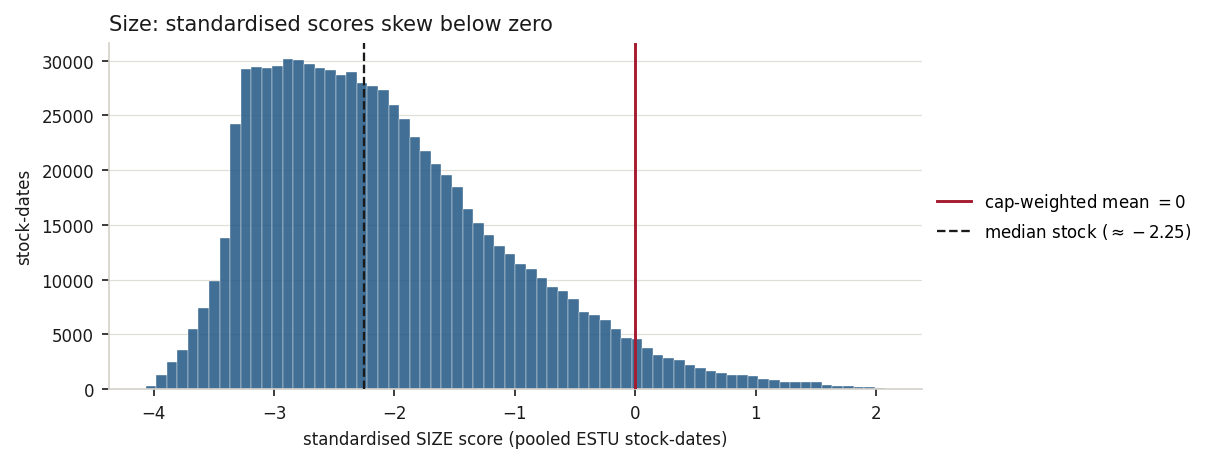
\includegraphics[width=\linewidth]{figures/size_score_dist.png}
\caption{The Size signature, pooled over all in-ESTU stock-dates. Standardisation sets the \emph{cap-weighted} mean to zero (red), but that center is dominated by the mega-caps, so it sits far out on the right tail; the typical (median) stock standardises near $-2.25$ (dashed), and only $\approx 80\%$ of the ESTU lies within $[\pm 3]$. The left skew is the offset center, not fat tails.}
\label{fig:size_dist}
\end{figure}


\begin{remark}
The high month-over-month Spearman ($\rho\approx 0.997$) is a sanity check, not a coincidence: a firm's market cap changes slowly relative to the cross-section, so its size rank is among the most persistent of any style descriptor. A sudden rank break is far more likely a data problem than a real event.
\end{remark}

\begin{example}
Why $\approx80\%$ in $[\pm3]$ rather than the $\approx99.7\%$ a Gaussian $z$-score would give? The median score is $\approx-2.25$, so the lower band edge at $-3$ sits only about $0.75$ standard deviations below the median -- it bites into the left side of the bulk. The asymmetry is not fat tails; it is the offset center. Widen the universe to micro-caps and the in-band fraction falls further (to $\approx44\%$), because micro-caps pile up far below the cap-weighted center, pushing more mass past $-3$.
\end{example}

\begin{exercise}
Show that the standardised score $s_n$ is invariant to the units of $M_n$: replacing $M_n$ by $cM_n$ for a common constant $c>0$ leaves every $s_n$ unchanged. (Hint: $\ln(cM_n)=\ln c + \ell_n$; track what the constant does to $\mu_{\mathrm{cw}}$ in the numerator.)
\end{exercise}

\begin{exercise}
Explain why the ESTU median SIZE score ($\approx -2.25$) being so far below zero is consistent with, not contradicted by, an equal-weighted standard deviation of exactly $1$. (Hint: the std is computed about the equal-weighted mean, but the score is centered on the cap-weighted mean; how far apart are the two means in standard-deviation units?)
\end{exercise}

\begin{exercise}
Roughly $80\%$ of ESTU names lie within $[\pm 3]$, against $\approx 44\%$ across all coverage. Argue qualitatively why widening the universe to micro-caps \emph{lowers} the fraction inside the band. (Hint: micro-caps add mass far below the cap-weighted center; what does that do to the left tail relative to $-3$?)
\end{exercise}

\section{Summary, and one honest caveat}\label{sec:summary}

\paragraph{Learning objectives.}
\begin{itemize}[leftmargin=1.4em,topsep=2pt,itemsep=1pt]
  \item Reproduce the four-step Size pipeline from memory.
  \item State the total-vs-float limitation and the lever that would close it.
\end{itemize}

The whole factor is four steps: take \emph{total} market cap, take its natural \emph{log}, \emph{trim} the result around the equal-weighted mean with a band wide enough to spare real large caps, and \emph{standardise} to cap-weighted mean $0$ / equal-weighted std $1$ over the ESTU. The output is a slow-moving, asymmetric score whose zero is the market's cap-weighted size and whose median name sits well below it -- a signature intrinsic to log-cap, and the Size column of the exposure matrix the cross-sectional regression is run against. It also feeds the downstream non-linear size factor.

\begin{pitfall}
\textbf{Honest caveat: total, not float.} We use total market cap because the data source lacks free-float figures. Total cap counts shares that never trade -- founder, insider, and strategic holdings -- so it overstates the investable size of closely held firms, making a founder-controlled company look larger (more positive SIZE) than its tradable footprint warrants. The clean fix is not a modelling trick but a data one: procure free-float share counts and recompute $M_n$ on the floated share base. Until then, read SIZE for insider-heavy names with this bias in mind.
\end{pitfall}

\begin{center}\small\itshape
References: Menchero, Orr \& Wang (2011), \textit{The Barra US Equity Model (USE4)} --- Empirical Notes, Appendix A (descriptor definitions and weights) and Methodology Notes, Sec. 2.2--2.3 (outlier trimming and standardisation). ESTU treated as an MSCI USA IMI proxy.
\end{center}

\end{document}
